\chapter{Processi e metodologie}
\label{chap:processi-metodologie}

Lorem ipsum dolor sit amet, consectetuer adipiscing elit. Aenean commodo ligula eget dolor. Aenean massa. Cum sociis natoque\footnote{\cite{site:agile-manifesto}} penatibus et magnis dis parturient montes, nascetur ridiculus mus. Donec quam felis, ultricies nec\footnote{\cite{article:spooky}}, pellentesque eu, pretium quis, sem.

\begin{figure}[H]
    \centering
    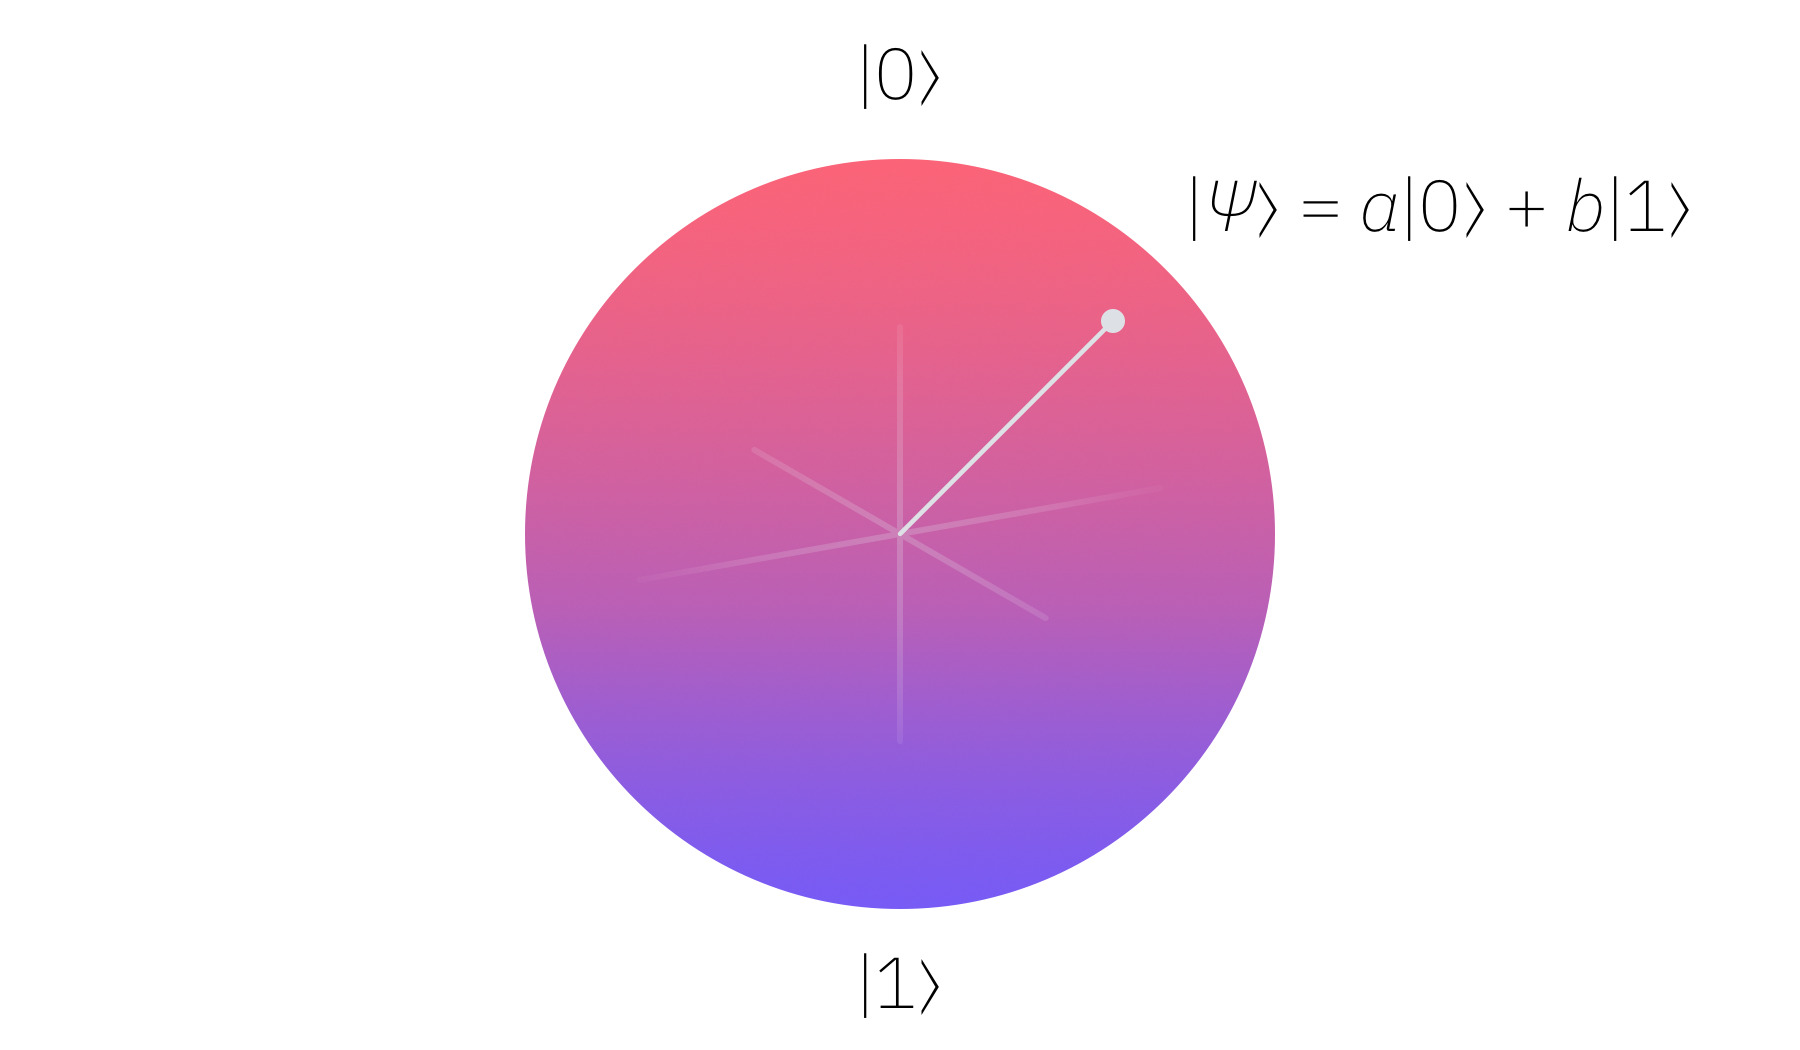
\includegraphics[alt={Testo alternativo dell'immagine}, height=5cm]{img/qubit.jpeg}
    \description[Rappresenzazione Qubit]{Long description}
    \caption{Lorem}
    \label{fig:qubit}
\end{figure}
\lipsum[1]

\section{Processo sviluppo prodotto}
\lipsum[1-2]

\begin{listing}[H]
\begin{minted}{c}
#include <stdio.h>
int main() {
    print("Hello, world!");
    return 0;
}
\end{minted}
\caption{Example of code}
\label{listing:b}
\end{listing}

Lorem ipsum:
\begin{listing}[H]
\begin{minted}{c}
#include <stdio.h>
int main() {
    print("Hello, world!");
    return 0;
}
\end{minted}
\caption{Example of code}
\label{listing:b-2}
\end{listing}

Lorem ipsum:
\begin{listing}[H]
\begin{minted}{c}
#include <stdio.h>
int main() {
    print("Hello, world!");
    return 0;
}
\end{minted}
\caption{Example of code}
\label{listing:b-3}
\end{listing}

\newpage